\chapter{Ingeniería de Software Ágil}

\section{Proceso de desarrollo}

Hacer agilidad no nos asegura calidad. Para ello primero hay que asegurarse de hacer ingeniería de software además de agilidad. Hay diferentes procesos de ingeniería o ciclos de vida y podemos tomar el siguiente: descubrimiento y definición de requerimientos (Discovery \& Requirements), análisis y diseño (Analysis \& Design), implementación y pruebas (Implementation \& Testing), integración y pruebas (Integration \& Testing), despliegue (Delivery) y "operación y monitoreo" (Operation \& Monitoring). En la última fase se contempla operaciones, monitoreo y el análisis de datos. Operaciones en cuanto a aseguramiento de la operatividad y rendimiento del software. El monitoreo de datos es el seguimiento a determinadas acciones que podemos cuantificar y que nos arrojaran datos relevantes para la estrategia (KPIs). Y el análisis de datos es la base de la optimización de la estrategia, que nos permite modificar, continuar o establecer nuevas directrices, sin perder de vista el objetivo final del software o producto.

\begin{figure}[h]
  \centering
  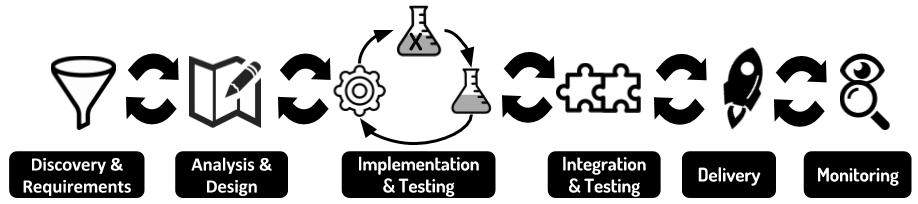
\includegraphics[width=0.99\textwidth]{PhasesOfSoftwareEngineering}
  \caption{Ciclo de ingeniería de Software}
  \centering
  \label{fig:PhasesOfSoftwareEngineering} %\ref{fig:PhasesOfSoftwareEngineering}
\end{figure}
\FloatBarrier % Command to control the position of floating images. With its, I can get the figures not to be pushed to the end of the document.
% El comando FloatBarrier es usado aqui para que la imagen se clave en este lugar y que no sea acarreada al final del documento.


Dicho esto, hay que considerar que el proceso de ingeniería de software ágil se hace sobre piezas de software (batch, feature o historia de usuario), y si bien es secuencial, tiene las fases del ciclo de vida que se solapan con las de otros piezas (ver fig. \ref{fig:PhasesOfSoftwareEngineering}). Es decir que el software se va desarrollando de a fragmentos o pequeñas piezas de software, en forma incremental y evolutiva. Cada pieza de software se desarrolla con diferentes instancias del ciclos de vida.

Correr este proceso bajo un marco ágil como Scrum, con prácticas ágiles es lo que podemos llamar ingeniería de software ágil (Agile Software Engineering). Además es conveniente introducir la idea de prácticas continuas, es decir refinamiento continuo (análisis y diseño con trabajo UX continuo), testing continuo (continuous testing), integración continua (continuous integration), despliegue o entrega continua (continuous deployment \& continuous delivery) y monitoreo continuo (continuous monitoring). 
Dicho esto, tenemos que tener en cuenta cómo unir y ajustar el proceso de ingeniería de software con el marco de trabajo Scrum. En este sentido es que se plantea ejecutar las fases del proceso de ingeniería, sobre historias de usuario, dentro del tren de sprints. En un equipo extremadamente autónomo y ágil, todas las fases se pueden desarrollar bajo el tren de sprints de Scrum.

\begin{figure}[h]
  \centering
  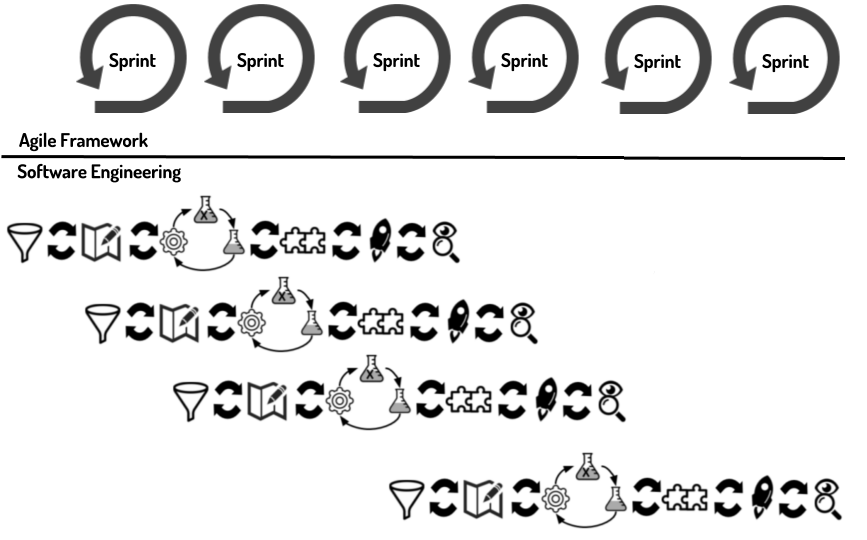
\includegraphics[width=0.99\textwidth]{AgileSoftwareEngineering}
  \caption{Ingeniería de Software Ágil}
  \centering
  \label{fig:AgileSoftwareEngineering} %\ref{fig:AgileSoftwareEngineering}
\end{figure}
\FloatBarrier % Command to control the position of floating images. With its, I can get the figures not to be pushed to the end of the document.
% El comando FloatBarrier es usado aqui para que la imagen se clave en este lugar y que no sea acarreada al final del documento.

De este modo, se integra el testing en fases más tempranas del desarrollo, por lo que QA no retrasa al equipo de desarrollo, porque QA está dentro del equipo y se trabaja con testing continuo. Los mismo sucede con UX y Operaciones.

\section{Testing continuo}

Si pensamos en Agile Testing pensamos en que queremos un testing dentro del equipo, con todo el equipo colaborando, que no sea solo una fase en un cascada, que reduzca el tiempo para recibir retroalimentación y asegure calidad suficiente. Cuando se incorpora agile testing, se introducen algunas prácticas, como por ejemplo Testing de “todo el equipo”, integración continua, testing guiado por pruebas (TDD), desarrollo guiado por pruebas de aceptación (ATDD), implementar la V de calidad usando historias, entre otros. 

\begin{figure}[h]
  \centering
  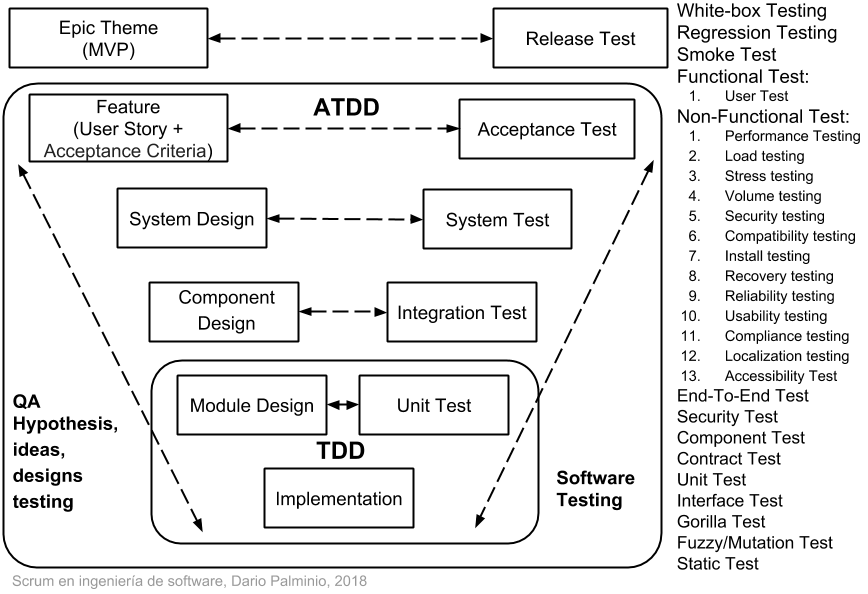
\includegraphics[width=0.99\textwidth]{AgileTesting_V}
  \caption{Modelo en V de calidad y testing}
  \centering
  \label{fig:AgileTesting_V} %\ref{fig:AgileTesting_V}
\end{figure}
\FloatBarrier % Command to control the position of floating images. With its, I can get the figures not to be pushed to the end of the document.
% El comando FloatBarrier es usado aqui para que la imagen se clave en este lugar y que no sea acarreada al final del documento.

Aunque considero que lo más importante es incorporar la mentalidad de testing continuo, independientemente de las prácticas o técnicas particulares.

\begin{figure}[h]
  \centering
  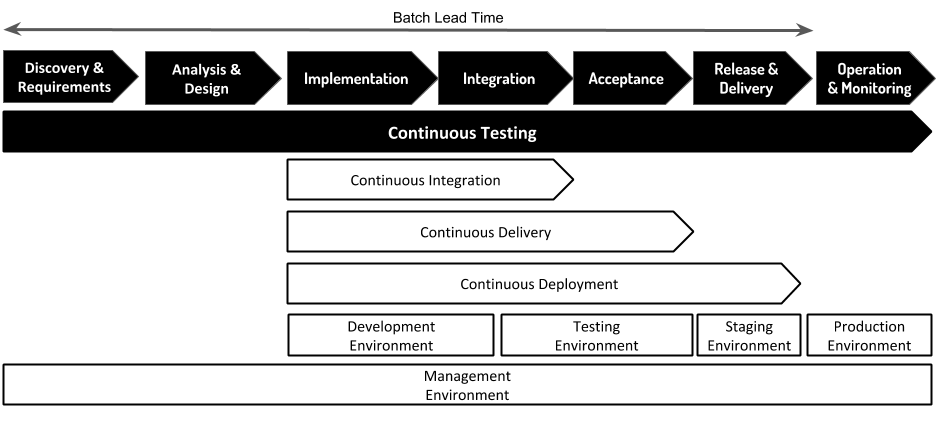
\includegraphics[width=0.99\textwidth]{structure_of_software_engineering_on_batch_life_cycle}
  \caption{Ciclo de vida de una historia y prácticas}
  \centering
  \label{fig:structure_of_software_engineering_on_batch_life_cycle} %\ref{fig:structure_of_software_engineering_on_batch_life_cycle}
\end{figure}
\FloatBarrier % Command to control the position of floating images. With its, I can get the figures not to be pushed to the end of the document.
% El comando FloatBarrier es usado aqui para que la imagen se clave en este lugar y que no sea acarreada al final del documento.

Cada fase del ciclo de vida del desarrollo puede contener prácticas de testing, desde las fases más tempranas hasta producción.

\begin{figure}[h]
  \centering
  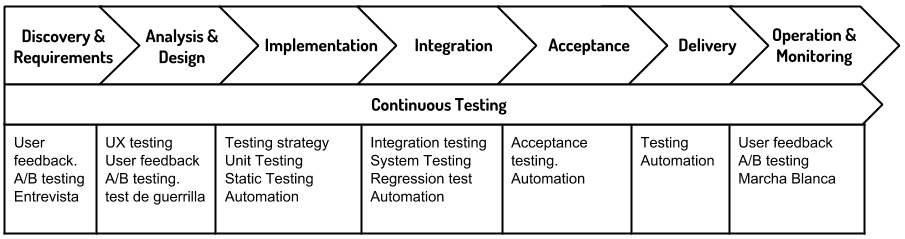
\includegraphics[width=0.99\textwidth]{continuous_testing_on_batch_life_cycle}
  \caption{Prácticas básicas en continuous testing}
  \centering
  \label{fig:continuous_testing_on_batch_life_cycle} %\ref{fig:continuous_testing_on_batch_life_cycle}
\end{figure}
\FloatBarrier % Command to control the position of floating images. With its, I can get the figures not to be pushed to the end of the document.
% El comando FloatBarrier es usado aqui para que la imagen se clave en este lugar y que no sea acarreada al final del documento.

Y, si lo pensamos bien, podemos decir que Scrum es una prueba de integración del sistema organizacional para validar continuamente si es posible que una organización entregue valor en un Sprint\footnote{Stacia Heimgartner Viscardi, Professional ScrumMaster's Handbook}. La prueba de Scrum revela los fallos de la organización, disfuncionalidades o los impedimentos que luego debemos buscar solucionar para lograr la agilidad organizacional. De este modo, cada Sprint que hagamos será un ciclo de testing organizacional, tanto de nuestro equipo como del resto de la organización, para levantar acciones de mejora que podemos explicitar, definir y evaluar en las sesiones de retrospectivas que tengamos y que apuntan a mejorar la propuesta de valor y el tiempo entre que se crea una historia y que la misma pueda ser validada por el cliente en forma operativa. Como dijo Jon Kern (co-autor del Manifiesto Ágil), “Ágil es reducir la brecha entre actuar y recibir feedback”, que en el desarrollo de productos se traduce a reducir el Time to Market (desde la perspectiva de negocio) o reducir el Delivery Lead Time (desde la perspectiva de DevOps); y Scrum nos ayuda a testear y medir esa brecha para reducirla. Con Scrum buscamos entregar software de calidad, que aporte valor, lo más pronto que sea posible.

\subsection{Tamaños de Testing}

Y hacia el equipo, el Scrum Master debe ayudarlo a que encuentre su manera de hacer buen testing y de mejorarlo. No existe realmente una forma única. Tampoco un convención de nombres y tipos de prueba claras. Depende de diferentes autores y de cada equipo. El Scrum Master debe ayudar con eso. Un ejemplo de esquema es el que han usado equipos en Google. A los desarrolladores de Google les gusta tomar decisiones basadas en datos, en lugar de confiar en el instinto o en algo que no se puede medir y evaluar. Ellos, llegaron a un acuerdo sobre un conjunto de convenciones de nomenclatura basadas en datos para sus pruebas. Llamaron a sus pruebas: "pequeñas", "medianas" y "grandes" \footnote{Test Sizes by Simon Stewart, Google Testing Blog, Monday, December 13, 2010.}. 

\begin{figure}[h]
  \centering
  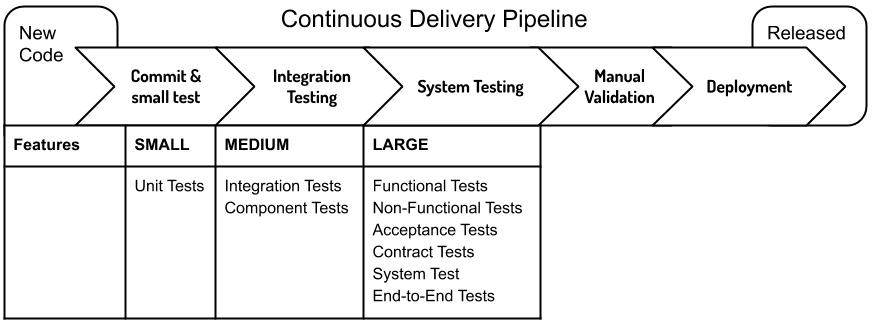
\includegraphics[width=0.99\textwidth]{Continuous_Delivery_Pipeline-small-medium-large}
  \caption{Tamaños de testing en el pipeline del Continuous Delivery}
  \centering
  \label{fig:Continuous_Delivery_Pipeline-small-medium-large} %\ref{fig:Continuous_Delivery_Pipeline-small-medium-large}
\end{figure}
\FloatBarrier % Command to control the position of floating images. With its, I can get the figures not to be pushed to the end of the document.
% El comando FloatBarrier es usado aqui para que la imagen se clave en este lugar y que no sea acarreada al final del documento.


Van de la prueba pequeña que equivale a una prueba de unidad, pasan por la prueba mediana que asegura que los niveles en la arquitectura de una aplicación pueden comunicarse correctamente y por una prueba grande que es una de extremo a extremo o de sistema.

\begin{figure}[h]
  \centering
  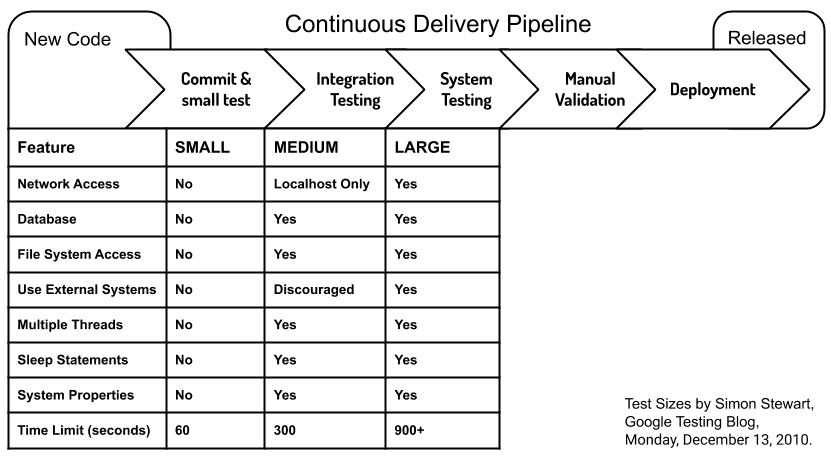
\includegraphics[width=0.99\textwidth]{TestingSize}
  \caption{Tamaños de testing y tipos en el pipeline del Continuous Delivery}
  \centering
  \label{fig:TestingSize} %\ref{fig:TestingSize}
\end{figure}
\FloatBarrier % Command to control the position of floating images. With its, I can get the figures not to be pushed to the end of the document.
% El comando FloatBarrier es usado aqui para que la imagen se clave en este lugar y que no sea acarreada al final del documento.


El Scrum Master debe asegurarse que el equipo encuentre la manera más efectiva y eficiente de hacer testing. Puede usar un esquema como el anterior, la pirámide de testing de Mike Cohn, la de Lisa Crispin o lo que encuentren apropiado. Sin testing de calidad no hay software de calidad.

\section{Prácticas técnicas}

Como ya he mencionado, es deseable que el SM vele por la excelencia técnica de su equipo y del proceso de desarrollo, buscando lograr un flujo limpio, cadenciosos y sostenible. Claro que la responsabilidad es del equipo y tanto un líder técnico como el SM, pueden liderar o guiar al equipo en el proceso de mejora continua del flujo de trabajo. Teniendo en cuenta las fases de desarrollo de los ítems de trabajo como historias, podemos tener dos aspectos en consideración para analizar el estado de nuestro procesos de desarrollo en cuanto a excelencia técnica. Por un lado, el aspecto de prácticas técnicas considerando la información, proceso, métodos, técnicas y organización (aquí se tiene en cuenta XP, DevOps, etc.). Por otro lado el aspecto tecnológico considerando las herramientas empleadas que cubren estas prácticas técnicas. Por ejemplo a continuación muestro un esquema de flujo y sus prácticas técnicas relacionadas.

\begin{figure}[h]
  \centering
  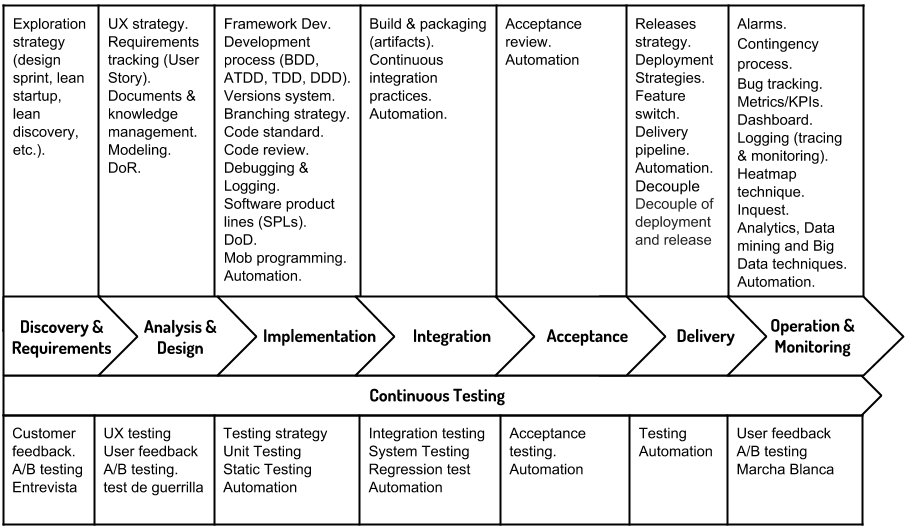
\includegraphics[width=0.99\textwidth]{practices_of_software_engineering}
  \caption{Flujo de prácticas técnicas}
  \centering
  \label{fig:practices_of_software_engineering} %\ref{fig:practices_of_software_engineering}
\end{figure}
\FloatBarrier % Command to control the position of floating images. With its, I can get the figures not to be pushed to the end of the document.
% El comando FloatBarrier es usado aqui para que la imagen se clave en este lugar y que no sea acarreada al final del documento.

Se puede hacer un esquema de flujo (el pipeline de producto o de delivery) semejante con los aspecto tecnológico, de herramientas, correspondientes a cada fase. Si bien hay un flujo genérico, cada equipo determinará cuál es su flujo y, en consecuencia, su pipeline.

\begin{figure}[h]
  \centering
  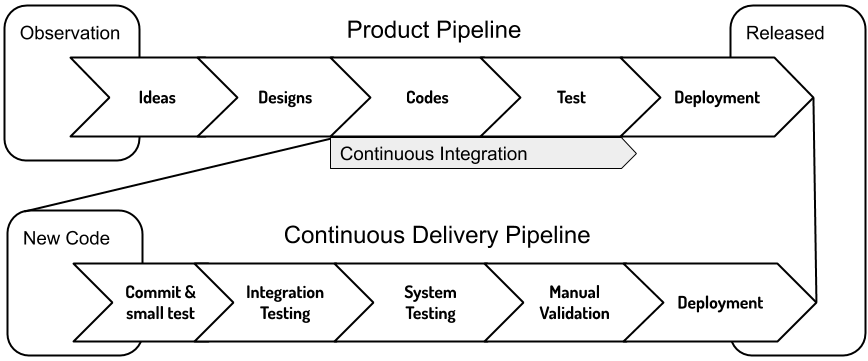
\includegraphics[width=0.99\textwidth]{Product_Pipeline}
  \caption{Flujo de producto vs. de delivery}
  \centering
  \label{fig:Product_Pipeline} %\ref{fig:Product_Pipeline}
\end{figure}
\FloatBarrier % Command to control the position of floating images. With its, I can get the figures not to be pushed to the end of the document.
% El comando FloatBarrier es usado aqui para que la imagen se clave en este lugar y que no sea acarreada al final del documento.


Hay que tener en cuenta que para que el flujo de desarrollo de software fluya limpio y cadencioso, la experiencia del desarrollo debe ser memorable y fluida sobre una plataforma e infraestructura que la facilite. Es por esto que un equipo de desarrollo tiene interdependencia con equipos de operaciones e infraestructura y es parte del desafío de un equipo de alto rendimiento disminuir la brecha, empoderarse y facilitar la integración de ese área de conocimiento.

\begin{figure}[h]
  \centering
  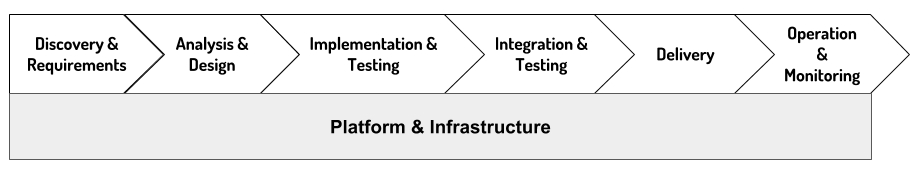
\includegraphics[width=0.99\textwidth]{Infrastructure}
  \caption{Plataforma e infraestructura}
  \centering
  \label{fig:Infrastructure} %\ref{fig:Infrastructure}
\end{figure}
\FloatBarrier % Command to control the position of floating images. With its, I can get the figures not to be pushed to the end of the document.
% El comando FloatBarrier es usado aqui para que la imagen se clave en este lugar y que no sea acarreada al final del documento.


\section{DevOps}

Nuestra mayor prioridad es satisfacer al cliente mediante la entrega temprana y continua de software útil y el enfoque DevOps nos ayuda a este objetivo. Aclaro aquí que DevOps no es más que una forma de especialización y de efoque dentro de la ingeniería de software. Por este motivo, una manera de deducir el nivel de ingeniería y, en consecuencia, de calidad de trabajo de un equipo es ver cómo se desenvuelven con DevOps en cuanto a cómo manejan la optimización y automatización del flujo de trabajo, la calidad y flexibilidad de su plataforma e infraestructura y como se integran o gestionan operaciones. A continuación veremos algunos temas de plataforma, infraestructura, pipeline, automatización y Feature toggles.


\subsection{Plataforma}


El trabajo de desarrollo de software es una actividad bastante compleja. Ya no se programa en texto plano y se integra enviando archivos por email. El trabajo del Scrum Master es ayudar a su equipo a que encuentre su stack tecnológico adecuado para el problema que intenta resolver. La complejidad de plataforma justa y mínima que facilite y optimice el flujo de desarrollo. Se debería preguntar: ¿Qué plataforma tiene y debería tener el equipo? ¿Cómo maneja o debería manejar la plataforma? ¿Cuáles son sus herramientas informáticas para idear, crear, integrar, probar, desplegar, monitorear y corregir errores de software de una manera ágil? ¿Cuán rápido permiten llevar una idea a producción?


Por ejemplo, un equipo estándar que desarrolla algún sitio web con una arquitectura orientada a microservicios. ¿Qué necesitaría? A modo de ejemplo podemos pensar en lo siguiente:
\begin{itemize}

\item \textbf{Análisis y diseño:} El equipo usará, en una de sus primeras fases, herramientas de gestión de proyectos (como Jira de Atlassian, Trello, etc.) para idear, definir, compartir, coordinar y planificar trabajo en forma de historias de usuario, tickets o docs. El equipo necesita comunicarse para lo que usará software de chatting (email, Slack, Rocket.Chat, Fleep, etc. ) y conferencias (Google Hangouts, Zoom, skype, etc.). En el proceso de análisis y diseño necesitará compartir documentación y otros archivos necesitando un repositorio de documentos compartidos (Google Drive, Dropbox, OneDrive y SharePoint en Office 36 de Microsoft, etc.). Sumando herramientas de diseño UX (por ejemplo para Wireframes, Visual Design, etc.) y de diseño y diagramado de software (Día, Visio, Google Draw.io, etc.). 

\item \textbf{Implementación:} En programación incluirán lenguajes, entornos IDE de programación (Eclipse, etc.) y librerías. Necesitará un gestor de configuración y versionado de software o Version Control System para trabajar en un código de propiedad compartida (github, Subversion, CVS, etc.). Para luego hacer sus push de código al repositorio.

\item \textbf{Integración:} Trabajará con un esquema de branching e integración de código para lo cual usará herramientas de compilación, dependencias y building, integración y despliegue (como Gitlab, Maven, etc.) además de herramientas de automatización de integración y despliegue (como Jenkins, Travis CI, Buildbot, DotCi, etc.). Aquí lo que hace es básicamente integrar en un ambiente aislado y posiblemente crear imágenes portables. También puede desplegar en ambientes de testing para luego correr las pruebas.

\item \textbf{Pruebas:} Junto a esto, para realmente hacer ingeniería, necesita herramientas de gestión, ejecución y automatización de pruebas (como Selenium, Sahi, Source Labs, Testing Bot etc.). Aquí ejecutará en un ambiente de testing pruebas automatizadas. También puede desplegar y testear en otros ambientes.

\item \textbf{Despliegue:} Herramientas para desplegar en producción (Jenkins, Travis CI, Buildbot, DotCi, Ansible, Puppet, Docker, etc.). Aquí se termina haciendo el despliegue a producción.

\item \textbf{Monitoreo:} Y, en su etapa de monitorear el software operativo en producción, necesita monitorear el rendimiento y la saludo del software y atender las contingencias que ocurran. Aquí necesitará herramientas de Bug-tracking como comunicación y sistema de ticket para identificaciones de errores y bugs (Bugzila, Mantis Bug Tracker, etc.), herramienta de logs o  registros y monitoreo (Splunk, Sumo Logic, LogStash, GrayLog, Loggly, PaperTrails, etc.). Y por último el equipo necesita evaluar los datos del negocio que opera el software, tendencias, comportamientos de los usuarios y clientes, para lo que puede usar herramientas de analítica digital y Business Intelligence (Splunk, Google Analytic, Elasticsearch y Kibana, Gafana, etc.).

\end{itemize}

La cantidad de pasos y despliegues dependerá de su pipeline, ambientes e infraestructura. Aquí nos podemos preguntar... ¿Sobre qué corren? ¿Sobre qué infraestructura funciona? ¿Qué ambientes de programación, pruebas y producción manejan? ¿Cuán versátil y fácil de configurar es? ¿Que dominio, propiedad y responsabilidad tiene el equipo sobre esta? ¿Cómo se comunican y se coordinan con los proveedores, admins y soportes?


\subsection{Infraestructura}


\subsubsection{Ambientes de software}
El flujo de desarrollo de software sucede y fluye por diferentes ambientes de software, que podrían clasificarse como ambiente de desarrollo local, de desarrollo compartido (o de integración), de prueba, de preparación (Staging) y de producción.

\begin{figure}[h]
  \centering
  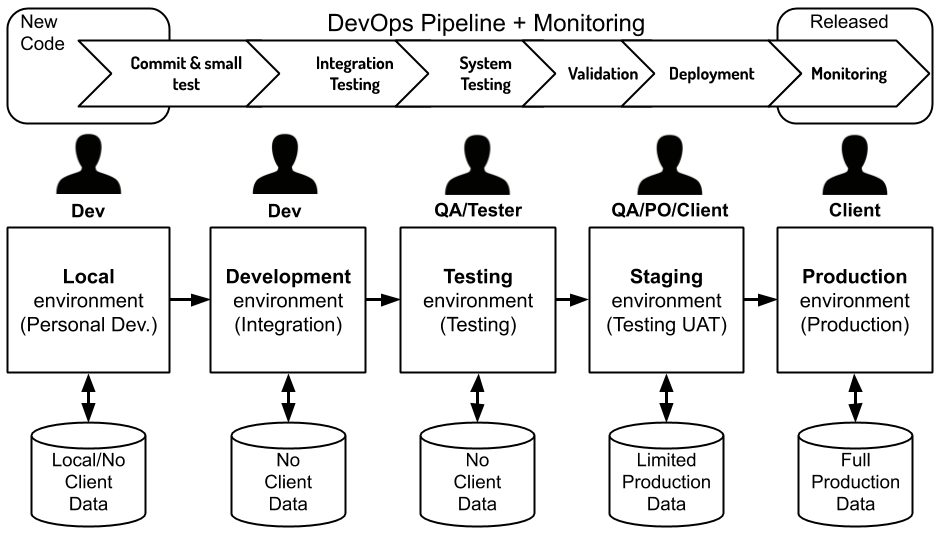
\includegraphics[width=0.99\textwidth]{Environment}
  \caption{Ambientes del flujo de desarrollo}
  \centering
  \label{fig:Environment} %\ref{fig:Environment}
\end{figure}
\FloatBarrier % Command to control the position of floating images. With its, I can get the figures not to be pushed to the end of the document.
% El comando FloatBarrier es usado aqui para que la imagen se clave en este lugar y que no sea acarreada al final del documento.

\begin{itemize}

\item \textbf{Desarrollo:} Un ambiente de desarrollo compartido e integración está configurado para permitir a los desarrolladores escribir código rápidamente, verificarlo creando pruebas básicas (pruebas unitarias) y ser productivo. Este entorno es mucho más pequeño de lo que se necesita para ejecutar una aplicación completa en una implementación de la vida real. También presenta herramientas específicas para desarrolladores que a veces pueden obstaculizar la validación rigurosa del control de calidad. Y lo más importante, el entorno de desarrollo cambia constantemente, con nuevas funciones que se agregan todo el tiempo, lo que dificulta que los ingenieros de control de calidad realicen pruebas que requieren mucho tiempo, pruebas de regresión o integración, sin interrumpir el proceso de desarrollo. Debido a que ejecutar pruebas complejas en el entorno de desarrollo conduciría a una gran pérdida de tiempo de los desarrolladores y, a su vez, por la poca estabilidad del software dificultaría el trabajo de los testers, es que se hace necesario otro entorno especializado para probar.

\item \textbf{Prueba:} El ambiente de prueba es donde los ingenieros de control de calidad pueden usar una variedad de herramientas de prueba para ejecutar todas sus diferentes pruebas sobre el código de aplicación tomado del entorno de desarrollo. Mientras los desarrolladores comprueban su código en busca de errores simples antes de pasarlo para garantizar la calidad, los testers ejecutan tipos de pruebas más complejas y que requieren mucho tiempo para verificar la compatibilidad del código nuevo y antiguo, la integración correcta de los diferentes módulos, el rendimiento del sistema, etc. 

\item \textbf{Staging:} Luego se necesitan pruebas de aceptación del usuario en un ambiente Staging, provisional, antes de subir a producción. El Staging es un entorno de ensayo pre-productivo y es una réplica idéntica del entorno de producción del cliente, que también suele contener datos de producción reales que se han desinfectado por motivos de seguridad. Está alojado de la misma manera que los servidores de producción e implica una configuración idéntica y operaciones de actualización. Por lo tanto, las pruebas en un entorno provisional ofrecen la forma más confiable de verificar la calidad del código y garantizar que los servidores de producción tengan éxito.

\item \textbf{Producción:} Y por último el ambiente productivo donde se explotará el software. Aquí estarán todos los datos reales del cliente y es donde el software, de algún modo, vive.

\end{itemize}

\subsubsection{Infraestructura ágil}
La infraestructura es como la autopista por donde circula nuestro código dentro de los ambientes como veículos. En consecuencia la calidad y tecnología de esta autopista determina la velocidad con que circulará nuestro código y la tasa de accidentes. La infraestructura ha evolucionado y seguirá haciéndolo a un ritmo acelerado. A continuación cuento una visión general de cómo se ha dado. 


\begin{figure}[h]
  \centering
  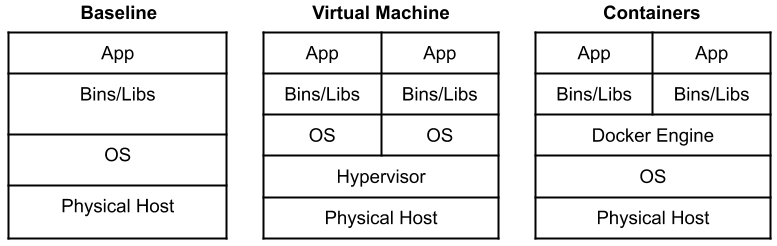
\includegraphics[width=0.99\textwidth]{Infrastructures}
  \caption{Infraestructura}
  \centering
  \label{fig:Infrastructures} %\ref{fig:Infrastructures}
\end{figure}
\FloatBarrier % Command to control the position of floating images. With its, I can get the figures not to be pushed to the end of the document.
% El comando FloatBarrier es usado aqui para que la imagen se clave en este lugar y que no sea acarreada al final del documento.

\begin{itemize}

\item \textbf{Baseline:} La forma más simple de infraestructura de trabajo que tenemos como desarrolladores es el Baseline, en donde el desarrollador instala todo lo necesario para programar y correr la aplicación desarrollada en su máquina física local. Y, además, puede usar servidores dedicados o Datacenters para hacer pruebas y despliegues. El problema de esta estrategia es que cuando estamos desarrollando una aplicación inestable puede desestabilizar todo el sistema, desconfigurar el computador y terminar todo en un caos provocado por la coexistencia de varios lenguajes o plataformas, librerías, servidores de bases de datos locales, espacios de trabajo de nuestro IDE, proyectos de versionado de código, etc… Y esto nos hace perder mucho tiempo en estabilizar todo de nuevo. Y en el caso de servidores compartidos esto se potencia, porque son más personas las que echan manos. Esto no es para nada ágil. Para mejorar esto surgió la posibilidad de trabajar con virtualización.

\item \textbf{Virtualización:} La virtualización nos permite ejecutar aplicaciones en un entorno controlado, con lo necesario para funcionar, encapsulado en un sistema operativo virtual independientemente de la máquina real que use. La virtualización funciona por medio de la abstracción de recursos, esto es por parte de un Hypervisor o VMM que corre en la máquina física del desarrollador. Una de las principales ventajas que tiene la virtualización es la capacidad de separar un entorno inestable (el virtual) de otro estable (la máquina física).  Esto permite restaurar el sistema a cualquier estado previo correcto en menos tiempo que si se trabajara directamente en la máquina física real como el caso Baseline. Otra ventaja es poder trabajar con múltiples entornos de prueba. Por ejemplo, en la misma máquina podemos correr la aplicación en distintos sistemas operativos. Esto mejora también el trabajo sobre servidores compartidos. Diferentes herramientas nos ofrecen virtualización de sistemas operativos (Docker, Virtuozzo, OpenVZ, Linux-VServer, etc.). Además existe la virtualización de procesos (Java Virtual Machine, etc.) y de sistemas (Oracle VM VirtualBox, MTL Virtual Machine, etc.). Junto a estas tecnologías surge la virtualización de red que nos ayuda a desacoplar completamente los recursos de red del hardware subyacente. El problema de la virtualización es que el proceso de configuración y distribución sigue siendo una tarea manual, repetitiva y en definitiva, poco conveniente. Esta forma no tiene tanta flexibilidad y portabilidad. Además, cuando necesitamos tener máquinas virtuales dedicadas y tenemos un elevado número de servidores en una misma máquina, se ve una clara reducción de recursos. Por eso surgió otra estrategia de virtualización más avanzada, la ‘containerización’.

\item \textbf{Containerización:} Los contenedores nos proporcionan un entorno aislado e independiente como forma de empaquetar todo lo necesario para ejecutar una aplicación: el código, las herramientas del sistema, librerías, etcétera. Sin usar sistemas operativos virtuales completos. Esto permite la portabilidad, que implica que los desarrolladores puedan crear aplicaciones en una computadora portátil y desplegarlas en los servidores, de forma más rápido, arrancarlas y pararlas más rápido y aprovechar mejor los recursos de hardware. Además facilita trabajar en una arquitectura de microservicios. Existen diferentes herramientas software que nos provee containerización (Kubernetes, Docker, Solaris Containers, etc.).

\item \textbf{Infraestructura como código:} Por otra parte, surge la “infraestructura como código”, en alternativa a la infraestructura tradicional que traía procesos manuales, errores humanos, demoras en configuraciones, cuellos de botella por entrega de la infraestructura, documentación incompleta, dificultad de introducir frecuentes cambios, etcétera. Con ella aplicamos herramientas y prácticas de ingeniería de software en nuestra infraestructura. Esto nos permite gestionar y proporcionar infraestructura de forma programática a través de código y automatización, para crear y cambiar servidores, instancias, entornos, contenedores o alguna otra infraestructura de forma ágil. En otras palabras, escribimos y ejecutamos código con diferentes herramientas software (Chef, Ansible de Redhat, Puppet, SaltStack, Terraform de HashiCorp, Vagrant, etc.) que define, despliega y actualiza infraestructuras.

\item \textbf{Cloud Computing:} Y todo esto nos lleva al Cloud Computing, o computación en la nube. Que es una plataforma que permite ofrecer las TI como servicios en la red. Todo lo que se encuentra en la nube Cloud se ofrece al usuario o programador como servicio, tanto software (SaaS), plataforma (PaaS) e infraestructuras (IaaS). El Cloud está basado en entornos virtualizados de alta disponibilidad y rendimiento sobre la infraestructura de Datacenter del proveedor. Además existe Elastic Computing que se aplica en los Elastic Cloud como tecnología de adaptación de uso de recursos en función de la demanda. Actualmente estas tecnologías son provista por proveedores dedicados al negocio de Clouding (Amazon, Azure, Google, Alibaba, etc.).

\end{itemize}


\subsection{Pipeline automatizado}

Desde el aspecto técnico, en ingeniería de software buscamos reducir el tiempo entre el inicio del desarrollo de una funcionalidad y su puesta en operaciones (lead time), la mejora continua de nuestro proceso de desarrollo de software y lograr código de calidad. Es decir acelerar el time-to-market, ser eficientes y entregar software de calidad que sea valioso para el cliente o el usuario. Y DevOps es parte de esta disciplina que se centra en efientizar todo el proceso desde el desarrollo hasta producción. En este sentido, podemos decir que el santo grial de DevOps es la automatización completa de todo el proceso centrándonos, de principio, desde que el desarrollador hace commit (push del código) hasta que su código llega a producción (Delivery Lead Time). El ideal de DevOps es lograr el "one click deployment": apretar una tecla y que llegue a producción. Para automatizar este proceso o flujo de despliegue, se necesita programar la generacón de código, integración, empaquetados, testing automáticos, orquestación, empaquetado y/o containerización y despliegue. Una manera de centralizar todo el flujo es en un “pipeline” y lo hacemos mediante la programación de configuraciones como scripts ("pipeline as code") usando algún “automation server” como Jenkins. 

\begin{figure}[h]
  \centering
  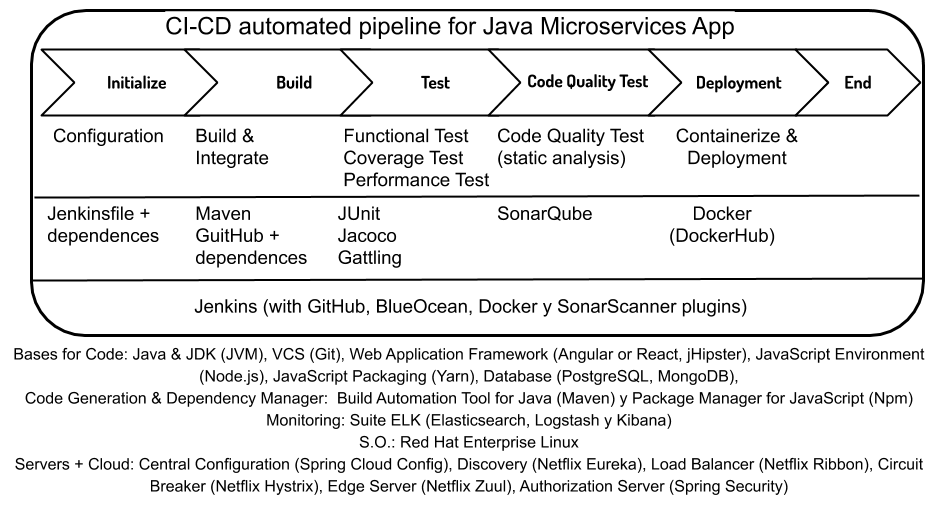
\includegraphics[width=0.99\textwidth]{CICDautomated_pipeline_forjava}
  \caption{Ejemplo de un CI-CD pipeline para una App Java con arquitectura de Microservicios}
  \centering
  \label{fig:CICDautomated_pipeline_forjava} %\ref{fig:CICDautomated_pipeline_forjava}
\end{figure}
\FloatBarrier % Command to control the position of floating images. With its, I can get the figures not to be pushed to the end of the document.
% El comando FloatBarrier es usado aqui para que la imagen se clave en este lugar y que no sea acarreada al final del documento.


Un pipeline es una secuencia de eventos o jobs que se pueden configurar y ejecutar como una secuencia de etapas STAGE. Donde cada STAGE es un conjunto de pasos Steps. Y cada Steps es una tarea que dice qué hacer mediante un bloque de líneas de código script.

\begin{figure}[h]
  \centering
  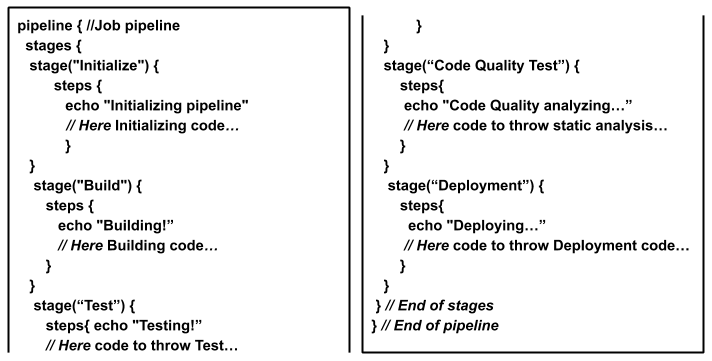
\includegraphics[width=0.99\textwidth]{CICDautomated_pipeline_forjava-code}
  \caption{Script ejemplo de un pipeline}
  \centering
  \label{fig:CICDautomated_pipeline_forjava-code} %\ref{fig:CICDautomated_pipeline_forjava-code}
\end{figure}
\FloatBarrier % Command to control the position of floating images. With its, I can get the figures not to be pushed to the end of the document.
% El comando FloatBarrier es usado aqui para que la imagen se clave en este lugar y que no sea acarreada al final del documento.

Cada pipeline que el equipo cree dependerá de su arquitectura de software, plataforma y la propia madurez de ingeniería de software del equipo. Y la arquitectura de software o la plataforma no es excusa para no hacer DevOps ni tener en cuenta un pipeline. Uses Java, Microsoft Visual Studio o SAP tu puedes hacer DevOps. Tal vez un  equipo más inmaduro en su desarrollo o al inicio de su proyecto tenga un pipeline pobre o no lo tenga. Y un equipo más desarrollado o avanzado tenga un pipeline más sofisticado (aunque simple de usar), rápido y automatizado. Tu pipeline demuestra tu nivel de DevOps y tu nivel de DevOps demuestra tu nivel de Ingeniería de Software. En particular recomiendo un pipeline basado en pruebas pequeñas (pruebas unitarias), medianas (pruebas de integración) y grandes (pruebas de sistema) y evolucionarlo de algo simple a algo más sofisticado y completamente automatizado. 

\begin{figure}[h]
  \centering
  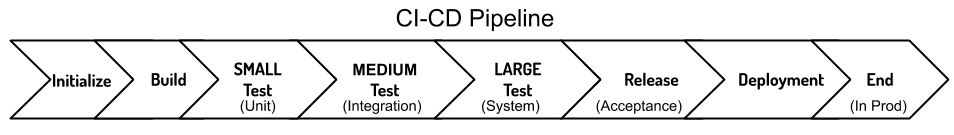
\includegraphics[width=0.99\textwidth]{CICDpipeline_small-medium-large}
  \caption{Esquema de un CI-CD pipeline tipo small-medium-large test}
  \centering
  \label{fig:CICDpipeline_small-medium-large} %\ref{fig:CICDpipeline_small-medium-large}
\end{figure}
\FloatBarrier % Command to control the position of floating images. With its, I can get the figures not to be pushed to the end of the document.
% El comando FloatBarrier es usado aqui para que la imagen se clave en este lugar y que no sea acarreada al final del documento.

\subsection{Activadores de características}

Algo contemplado en DevOps es la posibilidad de hacer rollback rápido o desactivar funcionalidades de forma simple y rápida. Algo que ayuda a esto y a desplegar rápidamente pequeñas funcionalidades es una técnica introducida por de "Feature Toggles" (feature switch o feature flag). Esta permite a los equipos modificar el comportamiento del sistema de software sin cambiar el código. Es como tener llaves de encendido de características de nuestra aplicación que corre en producción. Los Feature toggles se implementan con Feature Flags (vanderas de características). Y tenemos tres opciones básicas para implementar:

\begin{itemize}

\item \textbf{Static Feature Flag:} Esta es la manera más simple, pero menos recomendada, y consiste en usar variables banderas directamente en el código fuente y productivo como "toggle point" para habilitar o deshabilitar funcionalidades.

\item \textbf{Dynamic Feature Flag:} Otra manera es activar o desactivar flags de una manera dinámica fuera del código fuente core desde un subsistema que centraliza la configuración de flags y que se llama Toggle Configuration. Los  Toggle Configuration pueden ser archivos de configuración o config file (flags en archivos) o bases de datos (flags en tablas) con algún software de gestión de Feature Flags. Las aplicaciones tendrán características con Toggle Points que usan un Toggle Router para decidir según un Toggle Configuration externo. El Toggle Configuration y Toggle Router pueden evolucionar a subsistemas de administración más complejos, con interfaces de usuario y sistemas de autenticación.

\item \textbf{Context Flag:} Otro mecanismo es el que permite desactivar ciertas funciones para nuestra base general de usuarios en producción, pero poder activarla para usuarios internos. Esto se puede implementar usando configuradores de ambientes con Toggle Context. El Toggle Router leerá el ambiente de este Toggle Context y el Toggle Point encendera o apagará una característica según el contexto y el valor del Toggle Configuration.

\begin{figure}[h]
  \centering
  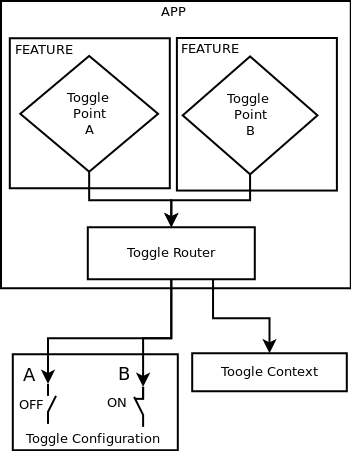
\includegraphics[width=0.55\textwidth]{Feature_Toggle}
  \caption{Esquema de feature toggle}
  \centering
  \label{fig:Feature_Toggle} %\ref{fig:Feature_Toggle}
\end{figure}
\FloatBarrier % Command to control the position of floating images. With its, I can get the figures not to be pushed to the end of the document.
% El comando FloatBarrier es usado aqui para que la imagen se clave en este lugar y que no sea acarreada al final del documento.

\item \textbf{Canary Releasing:} Esta técnica es una manera de incluir a la anterior. Consiste en permitir ir activando funcionalidades por zonas. Primero las activaríamos en sistemas internos, después en sistemas de clientes con confianza y si todo funciona correcto al final se activaría a todos o los clientes críticos. Si en alguna de estas zonas hay problemas, dejaríamos de avanzar y reestableceríamos el sistema para luego resolver el problema.

\begin{figure}[h]
  \centering
  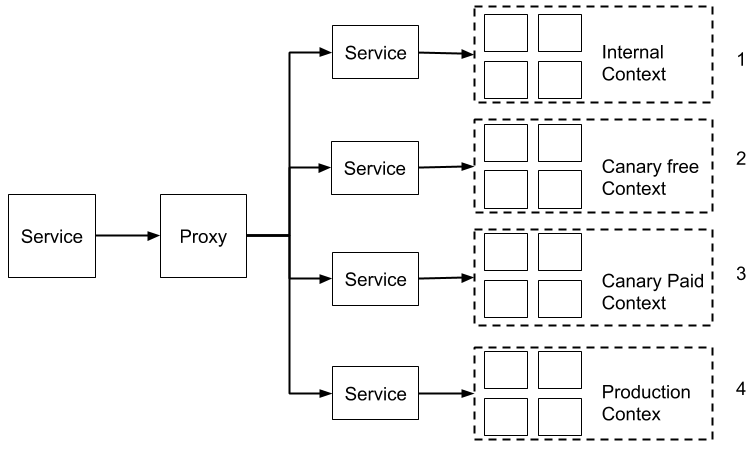
\includegraphics[width=0.90\textwidth]{canarycontext}
  \caption{Ejemplo de diferentes contextos para Canary Releasing}
  \centering
  \label{fig:canarycontext} %\ref{fig:canarycontext}
\end{figure}
\FloatBarrier % Command to control the position of floating images. With its, I can get the figures not to be pushed to the end of the document.
% El comando FloatBarrier es usado aqui para que la imagen se clave en este lugar y que no sea acarreada al final del documento.

\end{itemize}

Los Feature Flags ayudan a desplegar pequeños experimentos en producción para recibir feedback rápido, recuperar la estabilidad de la aplicación ante fallos fácilmente sin tener que desinstalar (sin hacer rollback), encender releases planificados desplegados apagados con anterioridad (solo encendiendo flags) y hacer pruebas por zonas de alcance de usuarios. Los Feature Flags impactan a las métricas de Deployment Frequency y MTTR mejorando la prestancia DevOps. Aunque no se debería abusar del uso de esta técnica. Se recomienda trabajar primero buscando desarrollar features lo más chicas posibles para hacer despliegues continuos de pequeñas funcionalidades. Y usar Feature Toggles solo cuando el equipo considere adecuado.

\section{En síntesis}

Hacer ingeniería de software ágil es desarrollar software de valor, de modo iterativo, incremental y evolutivo, con un producto o servicio que evoluciona, donde los requisitos y soluciones cambian con el tiempo, haciendo entregas frecuentes de calidad y valor, testeando continuamente, con feedback rápido, trabajando con equipos auto-organizados y multidisciplinarios que mejoran, inmersos en un proceso compartido de toma de decisiones interactiva y dinámica y entendiendo el negocio. Y, lo más importante, es considerar que la ingeniería es, además de una práctica científica, una práctica humana. Construir software se trata de relaciones humanas en un sistema social. Por eso, hay que construir relaciones humanas de valor, que habiliten la entrega continua de valor. Según Patrick Lencioni, un equipo humano debería tener ciertas aptitudes funcionales que posibilitan el trabajo de alto rendimiento: confianza, sin miedo al conflicto, compromiso, asunción de responsabilidades y atención a los resultados. Según el proyecto Aristóteles de Google, la clave es la cultura del equipo y lo necesario en ella es la seguridad psicológica entendida como: el sentimiento de confianza de que el equipo no va a avergonzar, rechazar o castigar a alguien por sus opiniones, comportamientos o ideas. Y como un equipo no es una isla, la organización que le da contexto debe reforzar este tipo de cultura, el factor humano, para lograr personas extraordinarias desarrollando resultados extraordinarios.
